\documentclass{article}
\usepackage[utf8]{inputenc}
\usepackage{tikz}

\title{TikZ}
\author{Pontus Vikstål}
\date{April 2019}

\begin{document}

%\maketitle

\newcommand\encircle[1]{%
  \tikz[baseline=(X.base)] 
    \node (X) [draw, shape=circle, inner sep=0] {\strut #1};}

\section{Introduction}

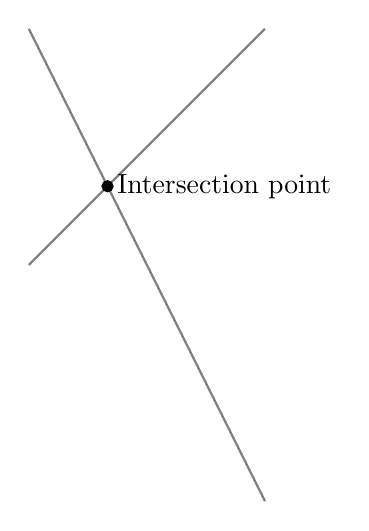
\begin{tikzpicture}
\draw[gray, thick] (-1,2) -- (2,-4);
\draw[gray, thick] (-1,-1) -- (2,2);
\filldraw[black] (0,0) circle (2pt) node[anchor=west] {Intersection point};
\end{tikzpicture}


\begin{tikzpicture}
\draw (-2,0) -- (2,0);
\filldraw [gray] (0,0) circle (2pt);
\draw (-2,-2) .. controls (0,0) .. (2,-2);
\draw (-2,2) .. controls (-1,0) and (1,0) .. (2,2);
\end{tikzpicture}

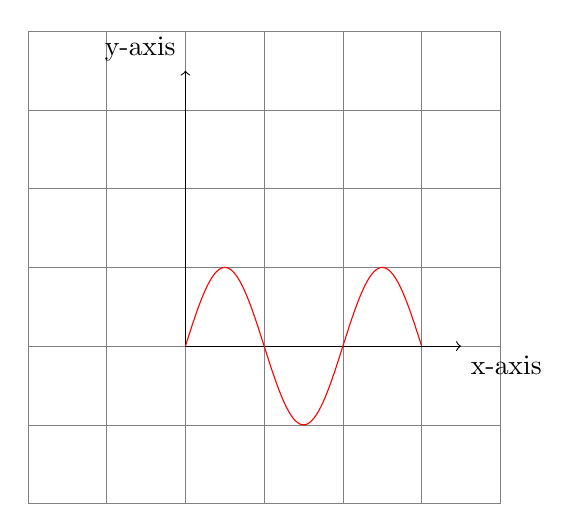
\begin{tikzpicture}
% grid
\draw [help lines] (-2,-2) grid (4,4);
% coordinate system
\draw[->] (0,0) -- (3.5,0) node[anchor=north west] {x-axis};  
\draw[->] (0,0) -- (0,3.5) node[anchor=south east] {y-axis};

% draw a sine curve. The trigonometric functions assume that x is in degrees; to express x in radians follow it with the notation "r"
\draw [red, domain=0:3, samples=100] plot (\x, {sin(pi*\x r)});

\end{tikzpicture}

% Bloch sphere
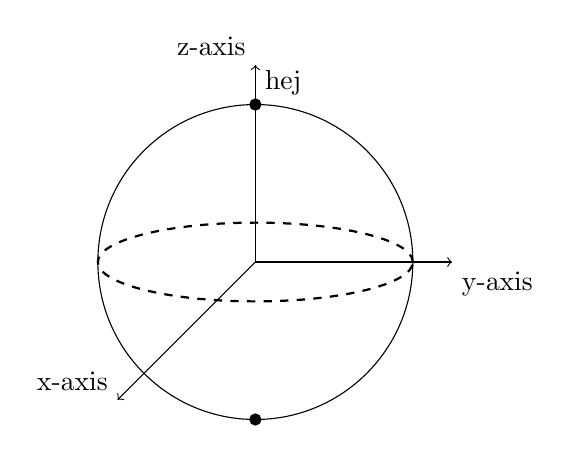
\begin{tikzpicture}
% circle
\draw (0,0) circle [radius=2];
% ellipse
\draw[thick,dashed] (0,0) ellipse [x radius=2cm, y radius=.5cm];
% coordinate system
\draw[->] (0,0) -- (-1.75,-1.75) node[anchor=south east] {x-axis};
\draw[->] (0,0) -- (2.5,0) node[anchor=north west] {y-axis};  
\draw[->] (0,0) -- (0,2.5) node[anchor=south east] {z-axis};

% points
\filldraw[black] (0,2) circle (2pt) node[anchor=south west] {hej};
\filldraw[black] (0,-2) circle (2pt);

\end{tikzpicture}
\end{document}
